

\newpage % Rozdziały zaczynamy od nowej strony.
\section{Implementacja gry Statki}

W poniższym rozdziale opisana została architektura aplikacji oraz opisane zostały kluczowe zaimplementowane klasy. Pozostałe ważne fragmenty kodu są dostępne w załączniku 1.

\subsection{Wybór technologii}

\subsubsection{Frontend}

 Do implementacji warstwy frontend wybrano framework Vue.js. Jest to jeden z wielu dostępnych frameworków JavaScript \cite{vuejs}. Został wybrany ze względu na swoją prostotę, dobrą dokumentację oraz fakt, że jest się go stosunkowo łatwo nauczyć w porównaniu do innych frameworków, na przykład React.js czy AngularJS \cite{whyChooseVue}.
Dodatkowym plusem jest też fakt, że aplikacje napisane przy pomocy Vue.js bardzo łatwo jest hostować za darmo na Github Pages. Frontend napisany na potrzeby tej pracy dostępny jest pod adresem \url{https://kalina559.github.io/battleships-game/}.

Repozytorium z projektem dostępne jest w serwisie GitHub, pod adresem \url{https://github.com/kalina559/battleships-game}
\subsubsection{Backend}

Warstwa backend jest potrzebna do wykonywania bardziej skomplikowanych obliczeń, takich jak kalkulowanie kolejnych ruchów z wykorzystaniem algorytmów decyzyjnych. Stan danej rozgrywki jest również przechowywany po stronie serwera - czyli naszego backendu. Teoretycznie możliwe byłoby pominięcie warstwy backend, ponieważ algorytmy wykorzystane w tej pracy nie są aż tak ciężkie obliczeniowo, ale nie jest to najlepszą praktyką. Przechowywanie stanu gry po stronie klienta również wiązałoby się z ryzykiem manipulacji przez gracza, na przykład poprzez konsolę dewelopera w przeglądarce.

Do implementacji wykorzystano technologię .NET w wersji 8.0. .NET to platforma programistyczna stworzona przez firmę Microsoft. Głównym językiem używanym w .NET jest C\#, ale Microsoft wspiera również F\# oraz Visual Basic \cite{whatisdotnet} \cite{dotnetlanguages}. Wybrany w poniższej pracy język programowania to C\#. Aplikacja stanowi RESTful (Representational state transfer) API, z którego może korzystać frontend, aby pobierać lub aktualizować aktualny stan rozgrywki. Backend jest hostowany za pomocą Azure App Service i jest dostępny pod adresem \url{https://battleshipswebapi.azurewebsites.net/api/}

Repozytorium z projektem dostępne jest w serwisie GitHub, pod adresem \url{https://github.com/kalina559/battleships-backend}
\subsubsection{Baza danych}

Założenia pracy wymagały zapewnienia możliwości zapisu przebiegu zakończonych rozgrywek, aby móc je później przeanalizować. W tym celu wykorzystano Azure Cosmos DB for NoSQL. Składa się ona z dwóch kontenerów - 'GameSessions' oraz 'TestGameSessions'. Dokonano takiego podziału aby odseparować dane generowane przez rozgrywki człowiek-algorytm oraz algorytm-algorytm. Rekordy zawierają dokumenty JSON, więc zdecydowano, że nie ma potrzeby stosowania relacyjnej bazy danych.

\subsection{Architektura aplikacji}

Jak widać na rysunku 5.1, komunikacja pomiędzy backendem i frontendem działa w obie strony - backend jest odpytywany przez frontend o obecny stan gry, a następnie może aktualizować ten stan na podstawie ruchów gracza. Po zakończonej rozgrywce aplikacja backend zapisuje stan gry w bazie danych, ale potem nie ma już do niego dostępu. Aby sprawdzić przebieg poprzednich rozgrywek, należy połączyć się bezpośrednio do bazy danych.

\begin{figure}[!h]
    \label{fig:architektura}
    \centering 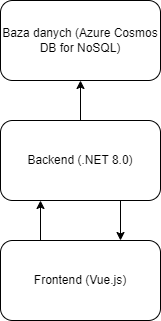
\includegraphics[width=0.2\linewidth]{img/architecture.drawio.png}
    \caption{Architektura aplikacji.}
\end{figure}

\subsection{Implementacja frontendu}
\indent Aplikacja frontend składa się z jednej strony, której zawartość zmienia się w zależności od wyborów gracza. Przed rozpoczęciem rozgrywki, gracz może wybrać zasady - czy statki mogą się ze sobą stykać czy też nie. Dropdown z wyborem algorytmu przeciwnika jest dostępny jedynie w lokalnie zbudowanej wersji aplikacji. Wersja produkcyjna, dostępna dla graczy, nie daje takiego wyboru. Dzięki temu gracze nie wiedzą z jakim algorytmem grają podczas rozstawiania swoich statków, nie wiedzą więc jakie rozstawienie byłoby dla nich najbardziej korzystne.

Dostępne są dwie wersje językowe aplikacji - polska oraz angielska.

\begin{figure}[!h]
    \label{fig:frontend-start}
    \centering 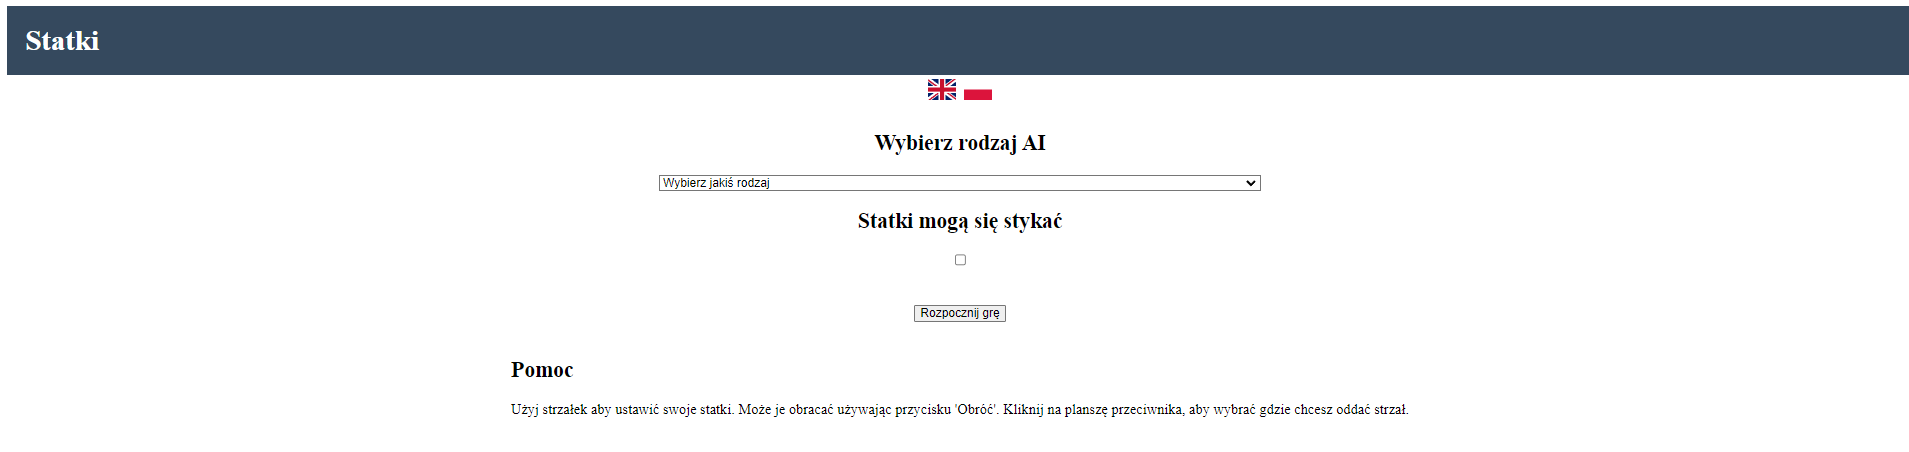
\includegraphics[width=1\linewidth]{img/frontend-start.PNG}
    \caption{Aplikacja frontend przed rozpoczęciem rozgrywki}
\end{figure}

Po kliknięciu przycisku "Rozpocznij grę", gracz widzi przed sobą dwie plansze, tak jak przedstawia to rysunek 5.2. Na górze znajduje się plansza przeciwnika, z niewidocznymi statkami, na dole zaś znajduje się plansza gracza, na której musi rozmieścić swoje statki. W tym celu użytkownik może skorzystać z przycisków znajdujących się pod swoją planszą. Rozwiązanie to zapewnia możliwość gry również na urządzeniach mobilnych, gdzie korzystanie ze strzałek na klawiaturze byłoby problematyczne.

\indent Na górze strony znajduje się element przedstawiający obecny stan gry - na rysunku 5.2 widnieje napis: "Czekanie na rozmieszczenie statków przez użytkownika". Ma to na celu zapewnienie graczowi informacji, co ma robić w danym momencie.

\begin{figure}[!h]
    \label{fig:frontend-game}
    \centering 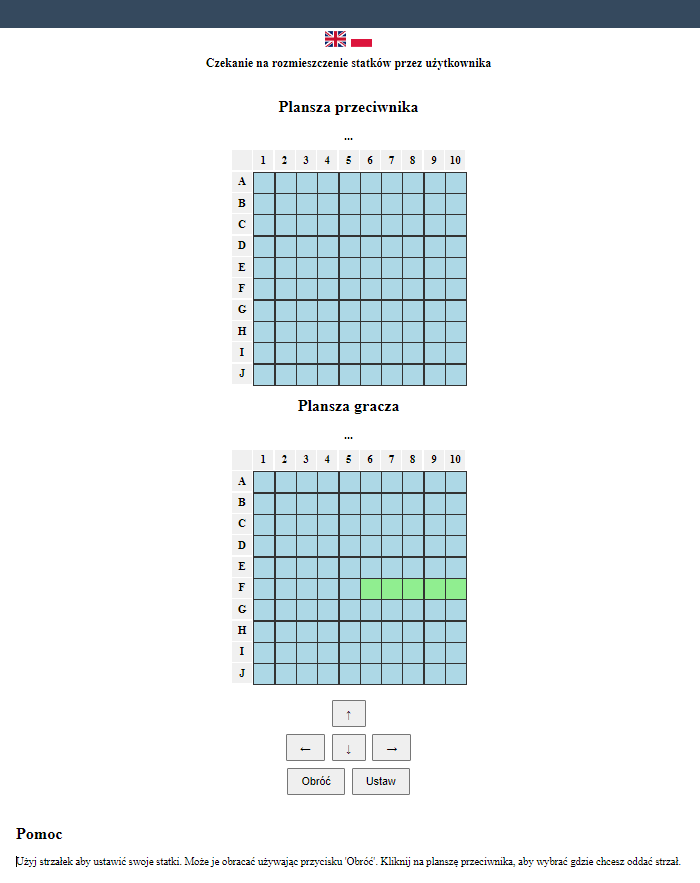
\includegraphics[width=1\linewidth]{img/frontend-game.PNG}
    \caption{Aplikacja frontend na starcie rozgrywki}
\end{figure}

Po rozstawieniu statków rozpoczyna się właściwa rozgrywka. Gracz i przeciwnik na zmianę oddają strzały, a nad ich planszami znajduje się informacja zwrotną o ostatnim strzale. Aby oddać strzał, gracz musi jedynie kliknąć w daną komórkę na planszy przeciwnika. Gra kończy się gdy wszystkie statki jednej ze stron zostaną zatopione. 

\begin{figure}[!h]
    \label{fig:frontend--in-game}
    \centering 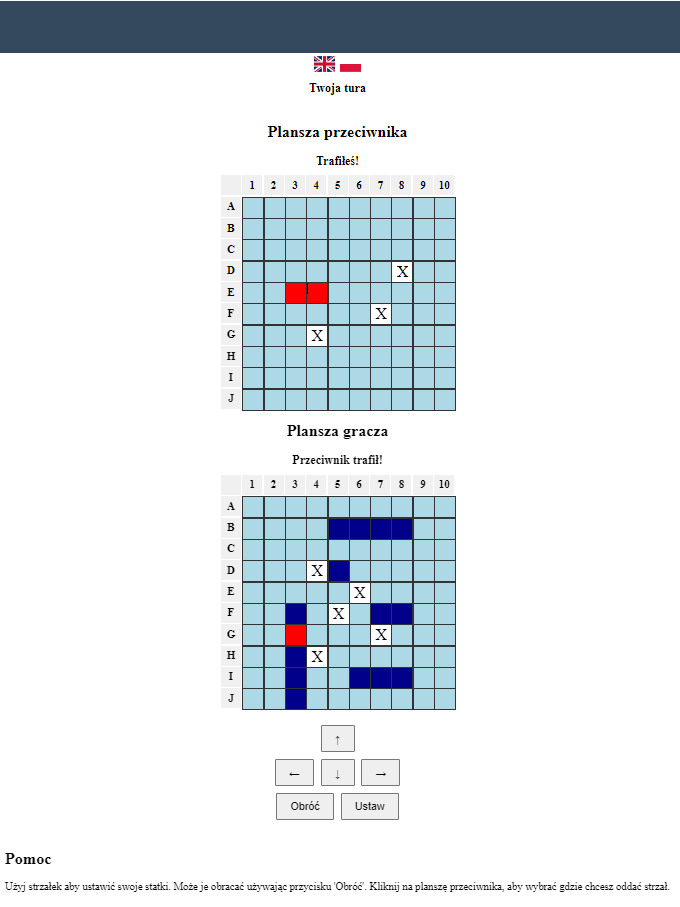
\includegraphics[width=1\linewidth]{img/frontend-in-game.PNG}
    \caption{Aplikacja frontend w trakcie rozgrywki}
\end{figure}

Aplikacja frontend składa się jedynie z kilku komponentów:
\begin{itemize}
    \item \textbf{Header.vue}: Tytuł strony "Statki", widoczny na rysunku 5.1.
    \item \textbf{Help.vue}: Wskazówki dla gracza, widoczne na dole rysunków 5.1, 5.2 i 5.3.
    \item \textbf{Menu.vue}: Menu z wyborem heurystyki oraz zasad, widoczne na rysunku 5.1.
    \item \textbf{OpponentGrid.vue}: Plansza przeciwnika, widoczna na rysunkach 5.2 i 5.3.
    \item \textbf{UserGrid.vue}: Plansza gracza, widoczna na rysunkach 5.2 i 5.3.
\end{itemize}

Plansze gracza i przeciwnika są oddzielnymi elementami, ponieważ różnią się zaimplementowaną logiką. Plansza przeciwnika przedstawia jedynie informacje płynące z backendu o tym, które pole zostało trafione i w które już strzelaliśmy. Plansza gracza zaś zapewnia możliwość rozstawienia statków. Z powyższych elementów korzysta główny komponent aplikacji, plik \emph{App.vue}.

Kluczowy jest też plik \emph{GameApi.js}, w którym zdefiniowany jest klient API oraz endpointy, które wołane są po stronie backendu.

Po otwarciu aplikacji w nowej przeglądarce zapisywany jest plik cookie 'sessionId', który następnie wysyłany jest z każdym zapytaniem do API. W ten sposób aplikacja backend wie, który gracz woła API i na tej podstawie aktualizuje stan danej gry. Projekty Web API w technologii .NET zapewniają podobną funkcjonalność, ale niestety, aby z niej skorzystać użytkownik musi wyrazić zgodę na "Pliki cookie innych firm" w przeglądarce. 

\subsection{Implementacja backendu}
\indent Aplikacja składa się z kilku projektów:
\begin{itemize}
    \item \textbf{Battleships.AI}: Zawiera heurystyki wykorzystywane do podejmowania decyzji przez przeciwnika.
    \item \textbf{Battleships.Common}: Zawiera klasy wykorzystywane w pozostałych projektach.
    \item \textbf{Battleships.Core}: Zawiera kluczowe dla aplikacji serwisy.
    \item \textbf{Battleships.UnitTests}: Zawiera testy jednostkowe, które zostały wykorzystane do testowania, która heurystyka jest najskuteczniejsza.
    \item \textbf{Battleships.WebApi}: RESTful API, które komunikuje się z frontendem. Zawiera kontrolery, do których wstrzyknięte za pomocą DI (Dependency injection) zostały serwisy z projektu Battleships.Core.
\end{itemize}

Endpointy, które zapewnia Battleships.WebApi.
\begin{itemize}
    \item \textbf{POST /api/AiType/list}: Zwraca listę algorytmów dostępnych do wyboru. Jest to endpoint typu POST, ponieważ do backendu przesyłana jest informacja jakie zasady wybrał gracz - czy statki mogą się ze sobą stykać. Używany na lokalnym środowisku.
    \item \textbf{POST /api/AiType/select}: Umożliwia graczowi wybór algorytmu decyzyjnego przeciwnika. Używany jedynie na lokalnym środowisku.
    \item \textbf{GET /api/GameState/get}: Zwraca obecny stan rozgrywki, a więc rozmieszczenie statków obu stron oraz dotychczasowe strzały.
    \item \textbf{GET /api/GameState/clear}: Umożliwia wyczyszczenie dotychczasowego stanu gry. Endpoint ten jest wołany po otwarciu gry, aby wyczyścić dotychczasową rozgrywkę - w ten sposób unikamy nieprzewidzianego zachowania aplikacji.
    \item \textbf{POST /api/Rules/update}: Umożliwia wybór zasad - czy statki mogą się ze sobą stykać, czy nie.
    \item \textbf{POST /api/ShipLocations/user}: Umożliwia graczowi rozmieszczenie statków. Endpoint ten jest wołany gdy użytkownik rozstawi wszystkie 5 swoich statków.
    \item \textbf{GET /api/ShipLocations/opponent}: Zwraca rozmieszczenie statków przeciwnika.
    \item \textbf{POST /api/Shot/user}: Umożliwia użytkownikowi oddanie strzału, wołany jest za każdym razem, gdy użytkownik w swojej turze wybierze komórkę na planszy przeciwnika.
    \item \textbf{GET /api/Shot/opponent}: Zwraca komórkę, którą algorytm decyzyjny przeciwnika wybrał do ostrzału.
\end{itemize}

Dokumentacja API dostępna jest pod adresem \url{https://battleshipswebapi.azurewebsites.net/swagger/index.html}.
\newline \newline
Najważniejszą klasą jest \emph{GameState}, widoczna na listingu 1. Wykorzystywana jest za każdym razem, gdy algorytm decyzyjny kalkuluje najbardziej korzystny ruch z punktu widzenia danej heurystyki. Dalej opisane zostaną klasy wykorzystane w \emph{GameState}. Klasa \emph{Ship}, widoczna na listingu 2, opisuje rozmiar, położenie oraz status statku. Klasa \emph{Shot}, widoczna na listingu 3, opisuje dany strzał - w jakie pole został oddany oraz czy trafiony został jakiś statek. Enum \emph{AiType} określa rodzaj heurystyki.

Pole \emph{PlayerAiType} jest wykorzystywane jedynie w testach jednostkowych, gdzie jako gracz występuje algorytm decyzyjny. Domyślnie jest puste, ponieważ w trakcie rozgrywki gracz-przeciwnik, to gracz podejmuje decyzje odnośnie strzałów.

\begin{addmargin}[10mm]{0mm}
\begin{lstlisting}[
    language={[Sharp]C},
    numbers=left,
    firstnumber=5,
    caption={Klasa GameState},
    aboveskip=0pt
]
public class GameState
{
    public List<Ship> UserShips { get; set; } = [];
    public List<Ship> OpponentShips { get; set; } = [];
    public List<Shot> PlayerShots { get; set; } = [];
    public List<Shot> OpponentShots { get; set; } = [];
    public AiType? PlayerAiType { get; set; } = null;
    public AiType OpponentAiType { get; set; }
    public bool ShipsCanTouch { get; set; }
}
\end{lstlisting}
\end{addmargin}

\begin{addmargin}[10mm]{0mm}
\begin{lstlisting}[
    language={[Sharp]C},
    numbers=left,
    firstnumber=3,
    caption={Klasa Ship},
    aboveskip=0pt
]
public class Ship
{
    public int Size { get; set; }
    public List<Coordinate> Coordinates { get; set; } = [];
    public bool IsSunk { get; set; } = false;
}
\end{lstlisting}
\end{addmargin}

\begin{addmargin}[10mm]{0mm}
\begin{lstlisting}[
    language={[Sharp]C},
    numbers=left,
    firstnumber=3,
    caption={Klasa Shot},
    aboveskip=0pt
]
public class Shot
{
    public int X { get; set; }
    public int Y { get; set; }
    public bool IsHit { get; set; }
}
\end{lstlisting}
\end{addmargin}

\begin{addmargin}[10mm]{0mm}
\begin{lstlisting}[
    language={[Sharp]C},
    numbers=left,
    firstnumber=3,
    caption={Enum AiType},
    aboveskip=0pt
]
public class Shot
public enum AiType
{
    Random = 0,
    RandomPlus = 1,

    LocationHeuristic = 2,
    LocationHeuristicDynamic = 3,
    HitHeuristic = 4,
    LocationAndHitHeuristic = 5,
    LocationAndHitHeuristicDynamic = 6,
}
\end{lstlisting}
\end{addmargin}

\subsection{Implementacja algorytmów decyzyjnych}
\indent Algorytmy decyzyjne w projekcie zostały zaimplementowane jedynie dla fazy gry, w której oddawane są strzały. Statki przeciwnika rozstawiane są zawsze losowo na planszy. W poniższym rozdziale wypisane zostały fragmenty kodu na najwyższym poziomie abstrakcji, bardziej dokładna analiza znajduje się w załączniku 1.

Wszystkie algorytmy są implementacją interfejsu IAiStrategy, przedstawionego na listingu 5.

\begin{addmargin}[10mm]{0mm}
\begin{lstlisting}[
    language={[Sharp]C},
    numbers=left,
    firstnumber=1,
    caption={Interfejs IAiStrategy},
    aboveskip=0pt
]
using Battleships.Common.GameClasses;

namespace Battleships.AI.Strategies
{
    public interface IAiStrategy
    {
        (int X, int Y) GenerateMove(
            List<Shot> previousShots,
            List<Ship> opponentShips,
            bool shipsCanTouch);
    }
}
\end{lstlisting}
\end{addmargin}

Algorytmy korzystające z heurystyk, dodatkowo dziedziczą po abstrakcyjnej klasie HeuristicStrategyBase, przedstawionej na listingu 6. Każdy taki algorytm musi implementować metodę GenerateProbabilityMap. Generowana przez tę metodę mapa prawdopodobieństwa określa jak duża jest szansa (według danej heurystyki), że na danej komórce znajduje się statek. Mapa jest listą par liczb (A,B), gdzie A określa współrzędne komórki, a B prawdopodobieństwo znajdowania się statku. W tym kontekście słowo 'prawdopodobieństwo' jest używane potocznie, a liczba B nie jest równa dokładnemu prawdopodobieństwu. Każda z heurystyk ma różne wagi i oblicza liczbę B w inny sposób, korzystając z umownych wartości.

\indent Na podstawie wygenerowanej mapy prawdopodobieństwa, algorytm wybiera najbardziej korzystny ruch. 

\begin{addmargin}[10mm]{0mm}
\begin{lstlisting}[
    language={[Sharp]C},
    numbers=left,
    firstnumber=9,
    caption={Abstrakcyjna klasa HeuristicStrategyBase},
    aboveskip=0pt
]
public abstract class HeuristicStrategyBase
    : IAiStrategy
{
    private static readonly Random _random = new();

    public (int X, int Y) GenerateMove(
        List<Shot> previousShots,
        List<Ship> opponentShips,
        bool shipsCanTouch)
    {
        var probabilityMap = GenerateProbabilityMap(
            previousShots,
            opponentShips,
            shipsCanTouch);

        var maxProbability = probabilityMap.Max();

        List<(int, int)> bestMoves = probabilityMap
            .Select((prob, index) => (prob, index))
            .Where(x => x.prob == maxProbability)
            .Select(x => (x.index % 10, x.index / 10))
            .Where(x => !previousShots
                .Any(shot => shot.X == x.Item1
                    && shot.Y == x.Item2))
            //make sure we're not shooting at
            //the same cell twice
            .ToList();

        if (bestMoves.Count != 0)
        {
            var move = bestMoves[_random.Next(bestMoves.Count)];
            return move;
        }

        // Fallback to a random move if no valid moves found
        // (shouldn't happen with a 10x10 grid)
        return new RandomStrategy().GenerateMove(
            previousShots,
            opponentShips,
            shipsCanTouch);
    }

    public abstract int[] GenerateProbabilityMap(
        List<Shot> previousShots,
        List<Ship> opponentShips,
        bool shipsCanTouch);
}
\end{lstlisting}
\end{addmargin}

\subsubsection{Algorytm losowy}
Najprostszy algorytm, w trakcie implementacji był traktowany jako grupa kontrolna - jeśli dany algorytm miał niższą skuteczność od algorytmu losowego, najprawdopodobniej wkradł się w niego jakiś błąd. Jedynym ograniczeniem przy wybieraniu komórki do ostrzału jest to, czy nie została już wcześniej ostrzelana.

\subsubsection{Rozszerzony algorytm losowy}
Dostępny jedynie gdy gracz wybierze opcję 'statki nie mogą się ze sobą stykać'. Różni się od zwykłego algorytmu losowego tym, że pomijane są pola, które sąsiadują z zatopionymi statkami.

\subsubsection{Algorytm oparty na heurystyce maksymalizacji zysku ze strzału}
Widoczny jest na listingu 7. Metoda \emph{AdjustProbabilityForShipLocations} dla każdego niezatopionego statku przeciwnika iteruje przez całą planszę i sprawdza czy początek statku może rozpoczynać się na danej komórce. Jako początek statku traktujemy jego współrzędną o najmniejszych współrzędnych X i Y. Możliwe położenie statku jest analizowane zarówno w pionie jak i w poziomie. Warunkami, które wykluczają możliwość rozpoczęcia się statku na danej komórce to:
\begin{itemize}
    \item (Jeśli użytkownik zaznaczył opcję 'statki nie mogą się ze sobą stykać'.) Jakakolwiek komórka sąsiadująca z możliwymi współrzędnymi statku została trafiona - czyli znajduje się na niej inny statek przeciwnika.
    \item Jakakolwiek komórka będąca możliwą współrzędną statku została już wcześniej ostrzelana.
    \item Jakakolwiek komórka będąca możliwą współrzędną statku została już wcześniej trafiona i jest częścią zatopionego statku.
\end{itemize}
Jeśli przykładowo statek o długości L może rozpoczynać się na komórce (X,Y) i leżeć w poziomie, to na mapie prawdopodobieństwa dodajemy liczbę 1 do komórek (X,Y), ..., (X+L, Y).


Metody \emph{AdjustProbabilityForSunkShips} oraz \emph{AdjustProbabilityForShotAtCells} są wykorzystywane również w pozostałych algorytmach opartych na heurystykach - służą one do wyzerowania wartości na mapie prawdopodobieństwa dla komórek, które zostały już ostrzelane lub sąsiadują z zatopionymi statkami (jeśli statki nie mogą się ze sobą stykać według zasad).

\begin{addmargin}[10mm]{0mm}
\begin{lstlisting}[
    language={[Sharp]C},
    numbers=left,
    firstnumber=9,
    caption={Klasa LocationHeuristicStrategy},
    aboveskip=0pt
]
public class LocationHeuristicStrategy
    : HeuristicStrategyBase
{
    private readonly static int
        POSSIBLE_SHIP_LOCATION_WEIGHT = 1;

    public override int[] GenerateProbabilityMap(
        List<Shot> previousShots,
        List<Ship> opponentShips,
        bool shipsCanTouch)
    {
        var probabilityMap = new int[100];

        HeuristicHelper.AdjustProbabilityForShipLocations(
            previousShots,
            opponentShips,
            shipsCanTouch,
            probabilityMap,
            POSSIBLE_SHIP_LOCATION_WEIGHT);

        if (!shipsCanTouch)
        {
            HeuristicHelper.AdjustProbabilityForSunkShips(
            opponentShips,
            probabilityMap);
        }

        HeuristicHelper.AdjustProbabilityForShotAtCells(
            previousShots,
            probabilityMap);

        GridHelper.PrintProbabilityGrid(probabilityMap, 10, 10);
        // just for debugging purposes

        return probabilityMap;
    }
}

\end{lstlisting}
\end{addmargin}

\subsubsection{Algorytm oparty na heurystyce najbardziej prawdopodobnej lokalizacji na podstawie trafień}
Algorytm jest widoczny na listingu 8. Metoda AdjustProbabilityForHitClusters znajduje dotychczasowe trafienia, które nie należą do zatopionych statków. W przypadku pojedynczych trafień, zwiększone zostają wartości na mapie prawdopodobieństwa dla komórek sąsiadujących w poziomie i w pionie z trafioną komórką. Jeśli znaleziona zostaje seria sąsiadujących trafień, zwiększone są wartości prawdopodobieństwa dla sąsiadujących komórek, znajdujących się na przedłużeniu tej serii. Wartość dodawana w tym przypadku ma większą wartość niż dla pojedynczych trafień.

\begin{addmargin}[10mm]{0mm}
\begin{lstlisting}[
    language={[Sharp]C},
    numbers=left,
    firstnumber=9,
    caption={Klasa HitHeuristicStrategy},
    aboveskip=0pt
]
public class HitHeuristicStrategy : HeuristicStrategyBase
{
    private readonly static int
        NEXT_TO_A_SINGLE_HIT_WEIGHT = 50,
        IN_LINE_WITH_OTHER_HITS_WEIGHT = 100;

    public override int[] GenerateProbabilityMap(
        List<Shot> previousShots,
        List<Ship> opponentShips,
        bool shipsCanTouch)
    {
        var probabilityMap = new int[100];

        HeuristicHelper.AdjustProbabilityForHitClusters(
            previousShots,
            opponentShips,
            probabilityMap,
            NEXT_TO_A_SINGLE_HIT_WEIGHT,
            IN_LINE_WITH_OTHER_HITS_WEIGHT);

        if (shipsCanTouch)
        {
            HeuristicHelper.AdjustProbabilityForSunkShips(
                opponentShips,
                probabilityMap);
        }

        HeuristicHelper.AdjustProbabilityForShotAtCells(
            previousShots,
            probabilityMap);

        GridHelper.PrintProbabilityGrid(probabilityMap, 10, 10);
        // just for debugging purposes

        return probabilityMap;
    }
}

\end{lstlisting}
\end{addmargin}

\subsubsection{Algorytm oparty na heurystyce maksymalizacji zysku priorytetyzującej dłuższe statki}
Właściwie identyczny do algorytmu opisanego w rozdziale 5.5.3. Jedyną różnicę pomiędzy algorytmami widać na listingu 9. Dla tego algorytmu zmienna dynamicWeight równa jest TRUE, a więc jeśli statek może znajdować się na danej komórce, to zamiast dodawać do niego zwykłą wagę, dodajemy wagę przemnożoną przez długość statku do potęgi dynamicPower (w tym przypadku 2). Wzór ten został już wspomniany w rozdziale 3.4, w punkcie 3.

\begin{addmargin}[10mm]{0mm}
\begin{lstlisting}[
    language={[Sharp]C},
    numbers=left,
    firstnumber=24,
    caption={Zwiększanie wartości na mapie prawdopodobieństwa dla algorytmu opartego na heurystyce maksymalizacji zysku priorytetyzującej dłuższe statki},
    aboveskip=0pt
]
probabilityMap[(y * 10) + x + i] += dynamicWeight
    ? weight * (int)Math.Pow(length, dynamicPower)
    : weight;
\end{lstlisting}
\end{addmargin}

\subsubsection{Algorytm oparty na heurystykach maksymalizacji zysku oraz najbardziej prawdopodobnej lokalizacji na podstawie trafień}
Kombinacja algorytmów z punktów 5.5.3 i 5.5.4. Znacznie większą wagę ma tu heurystyka najbardziej prawdopodobnej lokalizacji na podstawie trafień, a więc w praktyce heurystyka maksymalizacji zysku spełnia w pewnym sensie funkcję pomocniczą - wskazuje cele, jeśli żadna komórka nie została jeszcze trafiona, lub rozstrzyga, w którą z wielu komórek sąsiadujących z trafieniami najbardziej opłaca się strzelić, aby wyeliminować najwięcej możliwych położeń statków. Wszystkie metody widoczne w listingu 10 zostały opisane już we wcześniejszych punktach.

\begin{addmargin}[10mm]{0mm}
\begin{lstlisting}[
    language={[Sharp]C},
    numbers=left,
    firstnumber=10,
    caption={Klasa LocationAndHitHeuristicStrategy},
    aboveskip=0pt
]
    public class LocationAndHitHeuristicStrategy
        : HeuristicStrategyBase
    {
        private readonly static int
            POSSIBLE_SHIP_LOCATION_WEIGHT = 1,
            NEXT_TO_A_SINGLE_HIT_WEIGHT = 50,
            IN_LINE_WITH_OTHER_HITS_WEIGHT = 100;

        public override int[] GenerateProbabilityMap(
            List<Shot> previousShots,
            List<Ship> opponentShips,
            bool shipsCanTouch)
        {
            var probabilityMap = new int[100];

            HeuristicHelper.AdjustProbabilityForShipLocations(
                previousShots, opponentShips,
                shipsCanTouch,
                probabilityMap,
                POSSIBLE_SHIP_LOCATION_WEIGHT);

            HeuristicHelper.AdjustProbabilityForHitClusters(
                previousShots,
                opponentShips,
                probabilityMap,
                NEXT_TO_A_SINGLE_HIT_WEIGHT,
                IN_LINE_WITH_OTHER_HITS_WEIGHT);

            if (!shipsCanTouch)
            {
                HeuristicHelper.AdjustProbabilityForSunkShips(
                    opponentShips,
                    probabilityMap);
            }

            HeuristicHelper.AdjustProbabilityForShotAtCells(
                previousShots,
                probabilityMap);

            GridHelper.PrintProbabilityGrid(probabilityMap, 10, 10);
            // just for debugging purposes

            return probabilityMap;
        }
    }
\end{lstlisting}
\end{addmargin}

\subsubsection{Algorytm oparty na heurystykach maksymalizacji zysku oraz najbardziej prawdopodobnej lokalizacji na podstawie trafień priorytetyzującej dłuższe statki}
Bardzo podobna do punktu 5.5.6, z jedną różnicą - jeśli na planszy przeciwnika nie ma żadnego trafienia nienależącego do zatopionego statku, zamiast zwykłej heurystyki maksymalizacji zysku, stosujemy heurystykę maksymalizacji zysku priorytetyzującą dłuższe statki.

\begin{addmargin}[10mm]{0mm}
\begin{lstlisting}[
    language={[Sharp]C},
    numbers=left,
    firstnumber=10,
    caption={Klasa LocationAndHitHeuristicDynamicStrategy},
    aboveskip=0pt
]
public class LocationAndHitHeuristicDynamicStrategy
    : HeuristicStrategyBase
{
    private readonly static int
        POSSIBLE_SHIP_LOCATION_WEIGHT = 1,
        NEXT_TO_A_SINGLE_HIT_WEIGHT = 50,
        IN_LINE_WITH_OTHER_HITS_WEIGHT = 100;

    public override int[] GenerateProbabilityMap(
        List<Shot> previousShots,
        List<Ship> opponentShips,
        bool shipsCanTouch)
    {
        var probabilityMap = new int[100];

        var clusterCount =
        HeuristicHelper.AdjustProbabilityForHitClusters(
            previousShots,
            opponentShips,
            probabilityMap,
            NEXT_TO_A_SINGLE_HIT_WEIGHT,
            IN_LINE_WITH_OTHER_HITS_WEIGHT);

        if (clusterCount == 0)
        {
            HeuristicHelper.AdjustProbabilityForShipLocations(
                previousShots, opponentShips,
                shipsCanTouch,
                probabilityMap,
                POSSIBLE_SHIP_LOCATION_WEIGHT,
                dynamicWeight: true,
                dynamicPower: 2);
        }
        else
        {
            HeuristicHelper.AdjustProbabilityForShipLocations(
                previousShots,
                opponentShips,
                shipsCanTouch,
                probabilityMap,
                POSSIBLE_SHIP_LOCATION_WEIGHT);
        }

        if (!shipsCanTouch)
        {
            HeuristicHelper.AdjustProbabilityForSunkShips(
                opponentShips,
                probabilityMap);
        }

        HeuristicHelper.AdjustProbabilityForShotAtCells(
            previousShots,
            probabilityMap);

        GridHelper.PrintProbabilityGrid(probabilityMap, 10, 10);
        // just for debugging purposes

        return probabilityMap;
    }
}
\end{lstlisting}
\end{addmargin}
\indent